%%
%% Automatically generated file from Doconce source
%% (https://github.com/hplgit/doconce/)
%%





%-------------------- begin preamble ----------------------

\documentclass[%
twoside,                 % oneside: electronic viewing, twoside: printing
final,                   % or draft (marks overfull hboxes)
10pt]{article}


\listfiles               % print all files needed to compile this document


\usepackage{relsize,epsfig,makeidx,color,setspace,amsmath,amsfonts}
\usepackage[table]{xcolor}
\usepackage{bm,microtype}

\usepackage{minted,fancyvrb} % packages needed for verbatim environments


\usepackage[T1]{fontenc}
%\usepackage[latin1]{inputenc}
\usepackage[utf8]{inputenc}
% Set palatino as the default font family:
\usepackage[sc]{mathpazo}    % Palatino fonts
\linespread{1.05}            % Palatino needs extra line spread to look nice
\usepackage{lmodern}         % Latin Modern fonts derived from Computer Modern

% Hyperlinks in PDF:
\definecolor{linkcolor}{rgb}{0,0,0.4}
\usepackage[%
    colorlinks=true,
    linkcolor=linkcolor,
    urlcolor=linkcolor,
    citecolor=black,
    filecolor=black,
    %filecolor=blue,
    pdfmenubar=true,
    pdftoolbar=true,
    bookmarksdepth=3   % Uncomment (and tweak) for PDF bookmarks with more levels than the TOC
            ]{hyperref}
%\hyperbaseurl{}   % hyperlinks are relative to this root

\setcounter{tocdepth}{2}  % number chapter, section, subsection

% Tricks for having figures close to where they are defined:
% 1. define less restrictive rules for where to put figures
\setcounter{topnumber}{2}
\setcounter{bottomnumber}{2}
\setcounter{totalnumber}{4}
\renewcommand{\topfraction}{0.85}
\renewcommand{\bottomfraction}{0.85}
\renewcommand{\textfraction}{0.15}
\renewcommand{\floatpagefraction}{0.7}
% 2. ensure all figures are flushed before next section
\usepackage[section]{placeins}
% 3. enable begin{figure}[H] (often leads to ugly pagebreaks)
%\usepackage{float}\restylefloat{figure}

\usepackage[framemethod=TikZ]{mdframed}

% --- begin definitions of admonition environments ---

% Admonition is an oval gray box
\newmdenv[
  backgroundcolor=gray!5,  %% white with 5%% gray
  skipabove=\topsep,
  skipbelow=\topsep,
  outerlinewidth=0,
  leftmargin=0,
  rightmargin=0,
  roundcorner=5,
  needspace=0pt,
]{graybox1mdframed}

\newenvironment{graybox1admon}[1][]{
\begin{graybox1mdframed}[frametitle=#1]
}
{
\end{graybox1mdframed}
}

% --- end of definitions of admonition environments ---

% prevent orhpans and widows
\clubpenalty = 10000
\widowpenalty = 10000




% --- end of standard preamble for documents ---


% insert custom LaTeX commands...

\raggedbottom
\makeindex

%-------------------- end preamble ----------------------

\begin{document}



% ------------------- main content ----------------------



% ----------------- title -------------------------

\thispagestyle{empty}

\begin{center}
{\LARGE\bf
\begin{spacing}{1.25}
On Schemes for Exponential Decay
\end{spacing}
}
\end{center}

% ----------------- author(s) -------------------------

\begin{center}
{\bf Hans Petter Langtangen${}^{1, 2}$} \\ [0mm]
\end{center}

\begin{center}
% List of all institutions:
\centerline{{\small ${}^1$Center for Biomedical Computing, Simula Research Laboratory}}
\centerline{{\small ${}^2$Department of Informatics, University of Oslo}}
\end{center}
% ----------------- end author(s) -------------------------


\begin{center}
Jan 8, 2014
\end{center}

\vspace{1cm}



\begin{center}  % inline figure
  \centerline{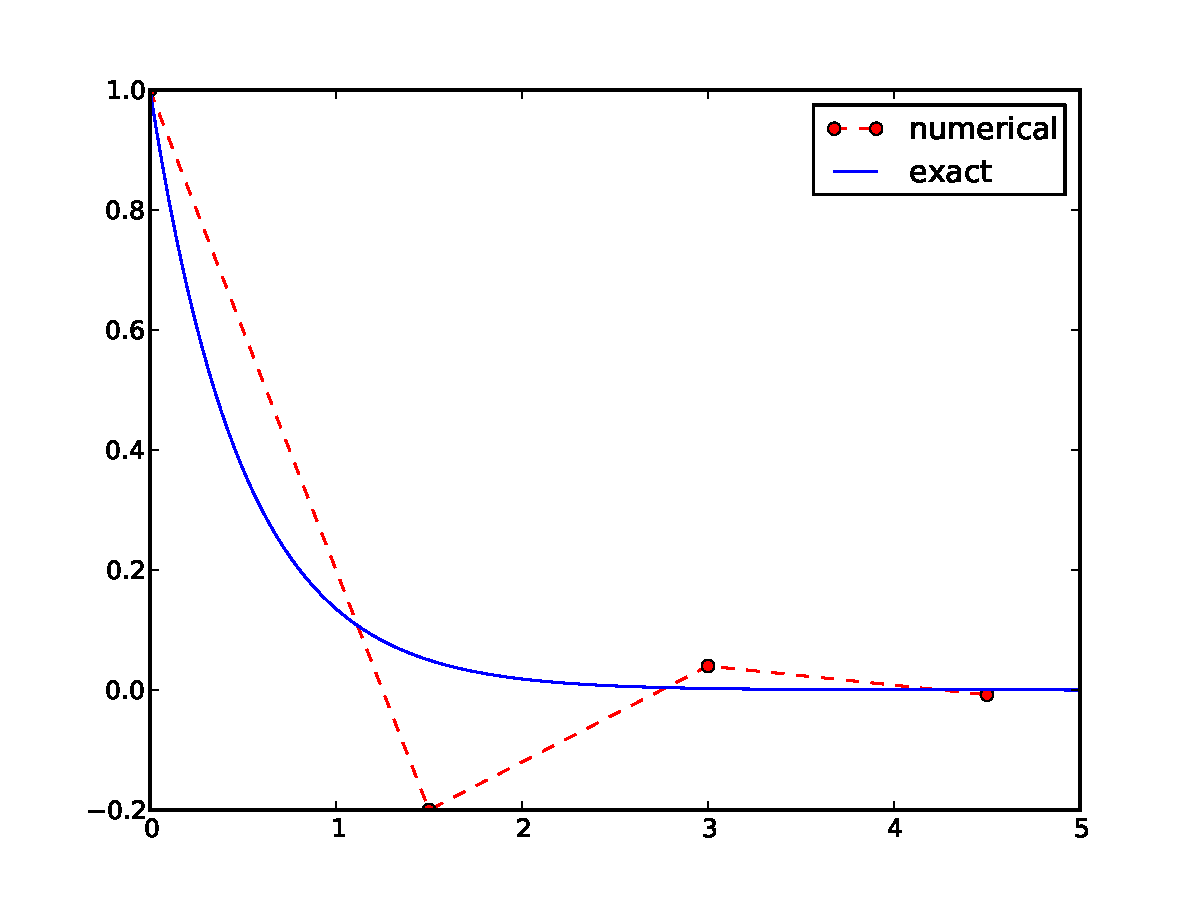
\includegraphics[width=0.4\linewidth]{fig/CN_logo.pdf}}
\end{center}



% !split

\section{Goal}

The primary goal of this demo talk is to demonstrate how to write
talks with \href{{https://github.com/hplgit/doconce}}{Doconce}
and get them rendered in numerous HTML formats.

\begin{graybox1admon}[Layout.]
This version
utilizes latex document slides with the theme \Verb!no theme!.
\end{graybox1admon}






% !bnotes
The talk investigates the accuracy of three finite difference
schemes for the ordinary differential equation $u'=-au$ with the
aid of numerical experiments. Numerical artifacts are in particular
demonstrated.
% !enotes


% !split
\section{Mathematical problem}


% !bslidecell 00


\begin{align}
u'(t) &= -au(t),
\label{ode}\\ 
u(0)  &= I,
\label{initial:value}
\end{align}

\begin{itemize}
 \item $t\in (0,T]$

 \item $a$, $I$, and $T$ are prescribed parameters

 \item $u(t)$ is the unknown function
\end{itemize}

\noindent
% !eslidecell


% !bslidecell 01

\begin{center}  % inline figure
  \centerline{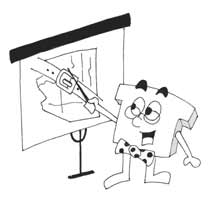
\includegraphics[width=0.5\linewidth]{fig/teacher2.jpg}}
\end{center}

% !eslidecell

% !split
\section{Numerical solution method}


% !bpop
\begin{itemize}
 \item Mesh in time: $0= t_0< t_1 \cdots < t_N=T$

 \item Assume constant $\Delta t = t_{n}-t_{n-1}$

 \item $u^n$: numerical approx to the exact solution at $t_n$
\end{itemize}

\noindent
% !epop

% !bpop
Numerical scheme:
   \[
   u^{n+1} = \frac{1 - (1-\theta) a\Delta t}{1 + \theta a\Delta t}u^n,
   \quad n=0,1,\ldots,N-1
   \]
% !epop


% !split

\section{Implementation}

The numerical method is implemented in a Python function:

\begin{minted}[fontsize=\fontsize{9pt}{9pt},linenos=false,mathescape,baselinestretch=1.0,fontfamily=tt,xleftmargin=7mm]{python}
def solver(I, a, T, dt, theta):
    """Solve u'=-a*u, u(0)=I, for t in (0,T] with steps of dt."""
    dt = float(dt)           # avoid integer division
    N = int(round(T/dt))     # no of time intervals
    T = N*dt                 # adjust T to fit time step dt
    u = zeros(N+1)           # array of u[n] values
    t = linspace(0, T, N+1)  # time mesh

    u[0] = I                 # assign initial condition
    for n in range(0, N):    # n=0,1,...,N-1
        u[n+1] = (1 - (1-theta)*a*dt)/(1 + theta*dt*a)*u[n]
    return u, t
\end{minted}

% !split
\subsection{The Crank-Nicolson method}



\begin{center}  % inline figure
  \centerline{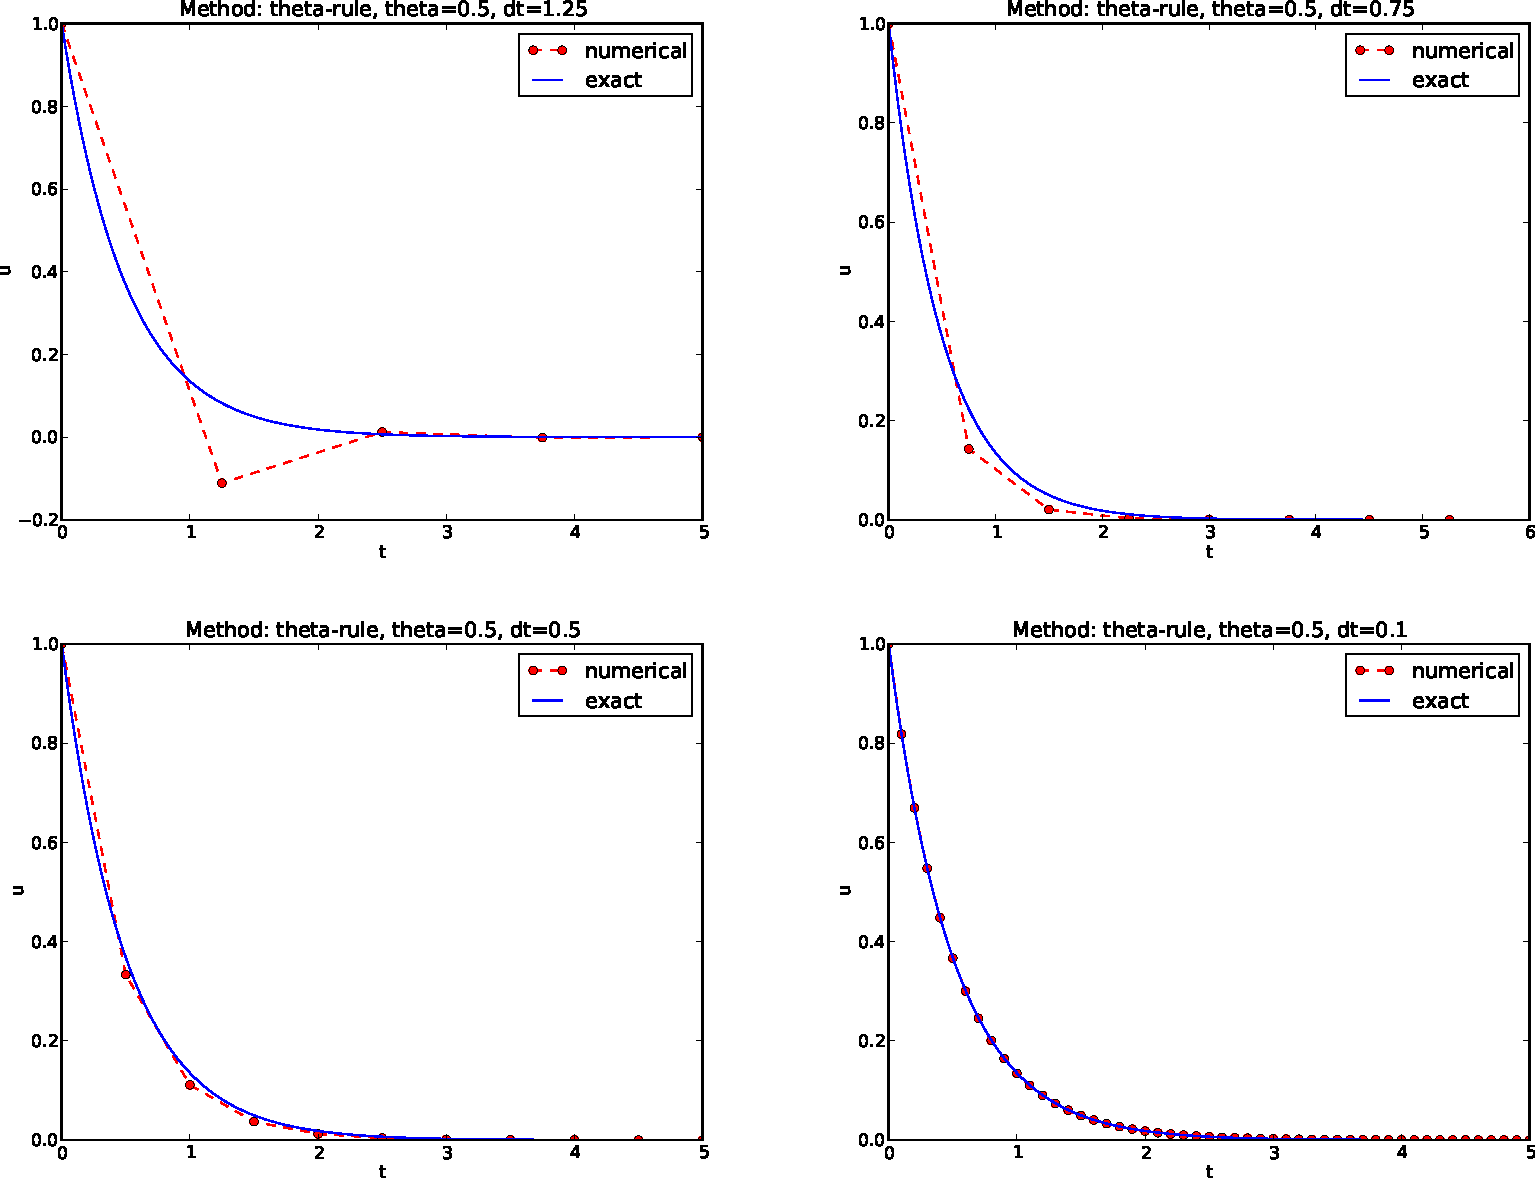
\includegraphics[width=0.9\linewidth]{fig/CN.pdf}}
\end{center}


% !split
\subsection{The artifacts can be explained by some theory}

% !bpop
Exact solution of the scheme:

\[ u^n = A^n,\quad A = \frac{1 - (1-\theta) a\Delta t}{1 + \theta a\Delta t}\thinspace .\]
% !epop

% !bpop
\begin{itemize}
 \item Stability: $|A| < 1$

 \item No oscillations: $A>0$

 \item Always for Backward Euler ($\theta=1$)

 \item $\Delta t < 1/a$ for Forward Euler ($\theta=0$)

 \item $\Delta t < 2/a$ for Crank-Nicolson ($\theta=1/2$)
\end{itemize}

\noindent
% !epop

% !bpop

\begin{graybox1admon}[Concluding remarks:]
Only the Backward Euler scheme is guaranteed to always give
qualitatively correct results.
\end{graybox1admon}


% !epop

% ------------------- end of main content ---------------


\printindex

\end{document}

